\section{Evaluation}
\label{sec:results}

Our evaluation asks three questions: (RQ1) \emph{Effectiveness}---can \sys produce clones that are behaviorally equivalent to their originals? (RQ2) \emph{Divergence}---are the generated clones structurally different enough to constitute genuine diversification rather than cosmetic edits? (RQ3) \emph{Cost}---how much verification effort, in repair iterations and tokens, does clone generation require? We answer them on the industrial measurement and control corpus described in Section~\ref{sec:impl}.

\subsection{Evaluation Corpus}

Table~\ref{tab:corpus} lists our subject programs. The corpus is designed around two axes that jointly isolate the contribution of each transformation agent. The first axis is \emph{transformation demand}, expressed as four categories: Category~A requires only a drop-in dependency swap (exercising the \emph{LSA}); Category~B additionally requires glue code to reconcile a new library's interface (exercising the \emph{GSA}); Category~C additionally requires rewriting first-party logic (exercising the \emph{LMA}), for example when the substitution removes a third-party control library and thereby turns its behavior into first-party code that must be diversified; and Category~D combines all three transformations within a single realistic program---an API-incompatible library swap, its integration glue, and substantial first-party control or estimation logic to diversify---so that the agents must cooperate end-to-end. The second axis is \emph{structural complexity}, ranging from a single self-contained module to multi-file packages with internal dependencies. All subjects are Python programs drawn from the industrial measurement and control domain, and each ships a \texttt{pytest} suite together with recorded input/output traces that serve as both the \emph{VCA}'s test corpus and the equivalence oracle's ground truth. In other words, the corpus supplies, per program, exactly the verification evidence \sys consumes.

Two subjects, \texttt{modbus\_meter\_reader} (B2) and \texttt{boiler\_control\_loop} (D1), declare a substitution that cannot be satisfied as stated: both originals speak Modbus TCP via \texttt{ModbusTcpClient(host, port=502)}, whereas the declared target \texttt{minimalmodbus} is serial-only and exposes no TCP entry point. We discovered this during evaluation rather than by design. Rather than repair the corpus we retained both as \emph{negative controls}, and they proved informative: across the nine \texttt{boiler\_control\_loop} runs, five independently selected \texttt{pyModbusTCP} over the declared target, and the single run that did adopt \texttt{minimalmodbus} was caught passing a TCP port number as a Modbus slave address.

\input{evaluation_programs}

\subsection{Metrics}

We define the following metrics before reporting results, so that success criteria are fixed independently of the outcomes.

\begin{itemize}
    \item \textbf{Generation success rate:} the fraction of subject programs for which \sys emits a clone that compiles and passes the full available test suite.
    \item \textbf{Equivalence-confirmation rate:} of the clones that pass local testing, the fraction the equivalence oracle certifies as semantically equivalent to the original. For the results reported here the oracle is the four-layer source-level checker described in Section~\ref{sec:impl}: import validation, recorded golden vectors at zero tolerance, program invariants, and the subject's own test suite. It is reported over Categories~C and~D only---the six subjects that ship golden vectors and invariants, giving eighteen runs per configuration. Categories~A and~B have no equivalence probes; scoring them as passes would present a test run as an equivalence proof.
    \item \textbf{Migration success:} an accepted clone. Stricter than generation success and used as the acceptance signal throughout: the clone compiles, passes its full suite and the oracle, the source genuinely changed, and the original dependency is verifiably absent. The last two conditions are necessary because every subject passes its own tests \emph{before} migration, so generation success alone cannot separate a real migration from an untouched file.
    \item \textbf{Structural divergence:} the degree to which the clone differs from the original, reported as the unweighted mean of two rename-insensitive measures taken between the delivered clone and the pristine original over the concatenation of all first-party files: the Ratcliff/Obershelp similarity of the pre-order AST \emph{node-type} sequence, which ignores identifier and literal choices, and a weighted Jaccard distance over a depth-tagged histogram of branch constructs, which captures reshaped control flow. The composite lies on $[0,1]$, higher meaning more divergent. We report a rename-insensitive measure deliberately: token-level edit distance rewards renaming every identifier, which is exactly the cosmetic change a Type~II detector defeats, and a diversification result that a detector defeats is not a result.
    \item \textbf{Repair cost:} the number of local execute-and-repair iterations per agent, and the number of \emph{VCA}-triggered stage re-entries, required to reach an accepted clone.
    \item \textbf{Token and monetary cost:} total tokens and estimated USD per generated clone.
    \item \textbf{Defect rate among accepted clones:} of the clones a configuration \emph{itself accepted}, the fraction an independent blind reviewer finds to carry \textsc{broken} or \textsc{major} behavioral defects (Section~\ref{sec:blindreview}). This measures the precision of a configuration's own success signal, which none of the automated measures above can assess.
\end{itemize}

\subsection{Experimental Setup}

We run \sys with \texttt{claude-sonnet-5} at temperature 0.7, three seeds per subject, a wall-clock ceiling of 180\,s per LLM request, and a cap of three \emph{VCA}-triggered stage re-entries per run, and record for each run whether generation succeeded, the metrics above, and the provenance report of applied substitutions and mutations. Temperature is deliberately not zero: the protocol calls for three runs per subject with different seeds so that variance can be reported, and at temperature zero those runs would be near-identical.

Every subject receives the same requirement: remove the dependency named in its \texttt{requirements.txt} while preserving observable behavior, and additionally, for Categories~C and~D, diversify all first-party logic. Crucially, \textbf{the replacement library is never named}---not to \sys and not to the baseline. Both must select a target themselves. An earlier protocol supplied the corpus's declared target to \sys while the baseline chose freely; that made the comparison asymmetric and, on the two negative controls, forced \sys toward a library that cannot work.

\paragraph{Baselines}
To isolate the contribution of \sys's agentic, verification-driven design, we compare against two configurations. \emph{Baseline~1 (single-shot LLM)} issues one prompt to the same model, naming only the dependency to be removed, with no agents, no tools and no verification loop; the reply is parsed for code blocks and used as-is. We verified by inspection and by telemetry that no tool loop is involved: exactly one LLM call on all 36 runs, averaging 1{,}471 input tokens, against up to 14 calls and 20{,}749 input tokens per run for full \sys. \emph{Baseline~2 (\sys without verification)} is an ablation with the \emph{VCA} and the global oracle disabled, leaving only the per-agent local execute-and-repair loop. These baselines let us attribute effectiveness gains to the two-tier verification discipline rather than to the underlying model.

\subsection{Results}

Table~\ref{tab:generation_results} reports the conventional measures. They do not separate the three configurations: generation success is 30/36, 33/36 and 29/36, and equivalence confirmation on Categories~C and~D is 16/18, 17/18 and 16/18. On these numbers alone the ablation is the strongest configuration and full \sys the weakest, which is the opposite of what the two-tier discipline predicts.

The measures are not wrong; they answer a narrower question than they appear to. Every subject's tests pass before migration, and every subject injects its I/O dependency, so the factory code that performs the substitution is frequently never executed by the suite. A clone can therefore compile, pass its full suite and satisfy the oracle while calling the new library incorrectly on the one path the tests do not reach. Compilation discriminates nothing at all: all three configurations compile on 36 of 36 runs.

\begin{table}[t]
\centering
\resizebox{\linewidth}{!}{%
\begin{tabular}{@{}lccccc@{}}
\toprule
\textbf{Configuration} &
\textbf{Gen.\ Success} &
\textbf{Equiv.\ Conf.} &
\textbf{Divergence} &
\textbf{Repair Iters} &
\textbf{Cost (USD)} \\
\midrule
Single-shot LLM (B1)       & 30/36 & 16/18 & 0.141 & 0 & \$0.79 \\
\sys w/o verification (B2) & 33/36 & 17/18 & 0.127 & 0 & \$3.87 \\
\sys (full)                & 29/36 & 16/18 & 0.154 & 6 & \$4.91 \\
\bottomrule
\end{tabular}%
}
\caption{Clone-generation results on the industrial measurement and control corpus. Twelve programs $\times$ three seeds $=$ 36 runs per configuration; equivalence confirmation is over Categories~C and~D only (18 runs per configuration). Repair iterations are \emph{VCA}-triggered stage re-entries, summed over all runs. \emph{Takeaway:} the conventional measures do not distinguish the three configurations---the ablation scores highest on two of them---which motivates the independent review reported in Table~\ref{tab:judge}.}
\label{tab:generation_results}
\end{table}

\subsubsection{Blind Review of Every Clone}
\label{sec:blindreview}

To measure what those instruments cannot, we submitted all 108 generated clones to a blind LLM review. Each clone was shown alongside its original to \texttt{claude-opus-5}---deliberately a different and stronger model than the \texttt{claude-sonnet-5} that generated it, so that no model grades its own output---and asked only for concrete behavioral differences, each naming a file, quoting a line and stating the runtime consequence. Style, structure and library choice are excluded explicitly. Verdicts are \textsc{broken} (fails on ordinary input), \textsc{major} (wrong behavior in a case the original handled), or \textsc{minor} (a real difference confined to an edge case). All system-identifying markers were renamed or removed before review, and the batch aborts rather than continuing if any marker survives, so the reviewer never learns which configuration produced a clone. \textsc{no-op} denotes a clone byte-identical to its original: trivially faithful because nothing was attempted, and therefore excluded from the clean rate rather than counted as a success.

\begin{table}[t]
\centering
\resizebox{\linewidth}{!}{%
\begin{tabular}{@{}lcccccc@{}}
\toprule
\textbf{Configuration} & \textsc{broken} & \textsc{major} & \textsc{minor} & \textsc{clean} & \textsc{no-op} & \textbf{Clean rate} \\
\midrule
Single-shot LLM (B1)       & 2 & 16 & 12 & 5  & 0  & 5/35 \\
\sys w/o verification (B2) & 1 & 8  & 1  & 15 & 11 & 15/25 \\
\sys (full)                & 5 & 8  & 4  & 16 & 3  & 16/33 \\
\bottomrule
\end{tabular}%
}
\caption{Blind review of all 108 generated clones by an independent, stronger model with every system-identifying marker removed. The clean rate excludes \textsc{no-op} clones, which attempted nothing. One single-shot run has no verdict---the reviewer returned an empty completion on four attempts with exponential backoff---so that configuration's denominator is 35.}
\label{tab:judge}
\end{table}

\begin{table}[t]
\centering
\resizebox{\linewidth}{!}{%
\begin{tabular}{@{}lccc@{}}
\toprule
\textbf{Configuration} & \textbf{Clones accepted} & \textbf{With serious defects} & \textbf{Defect rate} \\
\midrule
Single-shot LLM (B1)       & 28/36 & 15 & \textbf{54\%} \\
\sys w/o verification (B2) & 11/36 & 6  & \textbf{55\%} \\
\sys (full)                & 15/36 & 5  & \textbf{33\%} \\
\bottomrule
\end{tabular}%
}
\caption{Precision of each configuration's own success signal. Of the clones a configuration certified as an accepted migration, the fraction the blind reviewer found to carry \textsc{broken} or \textsc{major} defects. Accepting more clones and accepting sound clones are different capabilities, and on this corpus they trade off against one another.}
\label{tab:precision}
\end{table}

\begin{figure}[t]
\centering
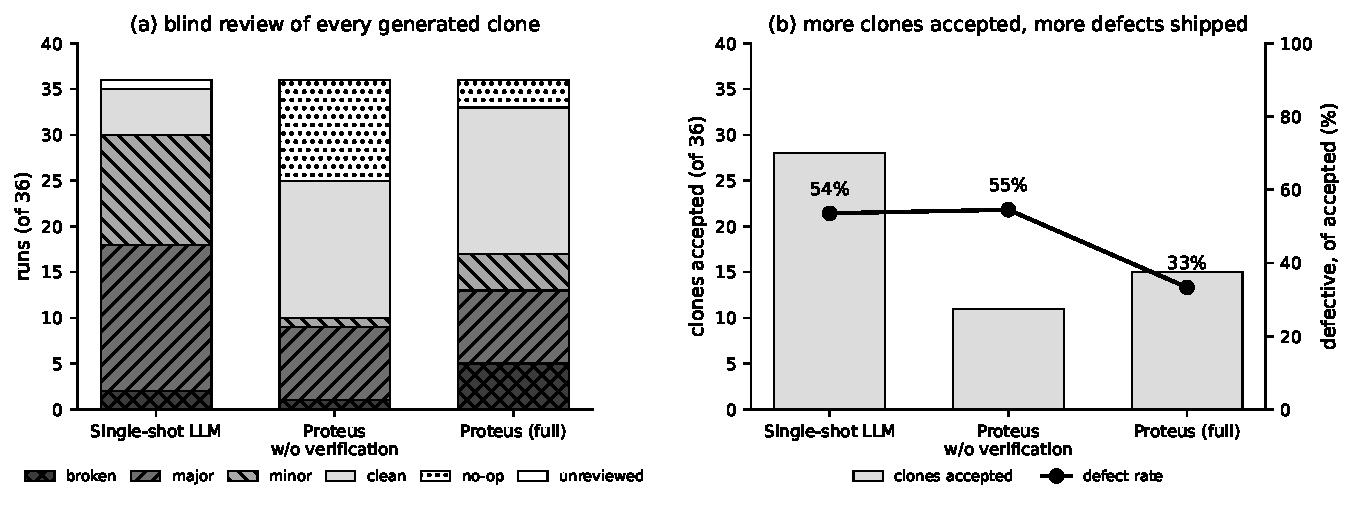
\includegraphics[width=\linewidth]{figs/results_figure.pdf}
\caption{(a) Every run classified by the blind reviewer. (b) The trade-off: the configuration accepting the most clones ships the highest fraction of defective ones. Read either panel alone and the ranking inverts, which is why both are shown.}
\label{fig:results}
\end{figure}

The review separates the configurations where the conventional measures do not (Table~\ref{tab:judge}, Table~\ref{tab:precision}, Fig.~\ref{fig:results}). Of the clones each configuration itself accepted, the fraction carrying \textsc{broken} or \textsc{major} defects is 54\% for the single-shot baseline, 55\% for the ablation, and 33\% for full \sys.

Two observations follow, and they point in opposite directions.

First, \textbf{the ablation performs like the single-shot baseline}: 55\% against 54\%. Removing the verification tier leaves an agent architecture no more reliable than a single prompt. Whatever \sys contributes is attributable to verification rather than to decomposition into cooperating agents.

Second, \textbf{full \sys does not deliver more sound clones than one prompt}. It yields 10 defect-free accepted clones per 36 runs against the baseline's 12. It accepts far fewer clones (15 against 28) and is right more often when it does accept---a precision gain paid for in recall. On a corpus where a wrong clone is worse than no clone, that is the trade we would choose, but it is a trade and not a dominance result.

\textbf{Cost.} The precision is not free. Full \sys consumed 925K tokens and 140 minutes across 36 runs against the baseline's 95K tokens and 6 minutes: roughly a sixfold increase in tokens and a twentyfold increase in wall time, for \$4.91 against \$0.79.

\textbf{Statistical caution.} With twelve subjects these differences are not statistically significant. Fisher's exact test gives $p=0.34$ for the single-shot baseline against full \sys on defect rate, and $p=1.00$ against the ablation; the 95\% confidence intervals overlap substantially (54\%~[36--70], 55\%~[28--79], 33\%~[15--58]). We report the direction and its mechanism, not a demonstrated effect. Separating 33\% from 54\% at $p<0.05$ would require roughly three to four times this corpus.

\subsection{Analysis}

\textbf{Which stage dominates repair cost.} Full \sys triggered six \emph{VCA} stage re-entries across 36 runs, all routed to the \emph{GSA}, and no run exhausted its repair budget. Repair cost is therefore not the binding constraint on this corpus; acceptance is.

\textbf{Which requirement classes are hardest.} The review's findings fall into a small number of recurring shapes, and the two systems fail differently. The single-shot baseline produces 80 findings dominated by \emph{fidelity} failures: 34 concern a changed exception type or message, and 10 concern a client or connection never closed. Its wiring is correct and its semantics drift. \sys produces 45 findings dominated by \emph{integration} failures: arguments accepted by an adapter and then never used (7 against the baseline's 2), adapters generated but not reached (5 against 2), and errors collapsed into a single generic exception (4 against 1). Its adapters are structurally sound---generating a wrapper naturally preserves lifecycle and error translation, which is why it has one unclosed resource against the baseline's ten---and it loses detail at the call sites.

\textbf{Characteristic failure modes.} In the ablation's \texttt{boiler\_control\_loop} clone, an adapter catches \texttt{(ModbusError, Exception)} and converts every failure---connection loss and programming errors such as \texttt{TypeError} alike---into a generic \texttt{IOError}. On a boiler supervisor an adapter bug becomes indistinguishable from a genuine Modbus fault. The ablation accepted this clone; full \sys rejected its counterpart at the \emph{VCA} on the same two seeds. In full \sys's own \texttt{boiler\_control\_loop} clone, the generated wrappers accept the per-call slave identifier and never use it, so an injected client configured for a different device would be actuated instead. Neither defect is reachable by the test suite, because the suite injects a fake client that ignores the same argument.

\textbf{What the global oracle catches.} Two \sys clones import the migrated-to library while still calling the migrated-from one, which was never imported---a guaranteed \texttt{NameError} on the factory path. Both were rejected by the pipeline, at the \emph{LMA} and the \emph{VCA} respectively, and the blind reviewer independently rated both \textsc{broken}. The system's own verdict and an independent reviewer's agree on precisely the clones the test suite passes.

\paragraph{Lessons Learned}
Three findings we did not anticipate.

\emph{Test suites are the wrong instrument for this task.} Dependency injection is good practice, and it makes the migrated code path untestable by the very suite that certifies it. Any future benchmark of clone generation needs an oracle that executes the substituted path directly, which is why we added factory execution as a fifth oracle layer mid-study.

\emph{Separating substitution from mutation keeps repairs local, but the seam leaks.} The \emph{LSA}/\emph{GSA} split behaves as intended---repairs stay within one agent and no run exhausted its budget---yet the residual failure mode lives precisely at the boundary, where an adapter is generated correctly and then not fully wired to the call sites it was written for. Orthogonal concerns still require a shared contract at their interface.

\emph{One third of the corpus is unsolved by every configuration.} Four subjects---the MQTT bridge, the PID controller, the threshold engine and the telemetry gateway---produced zero defect-free accepted clones across all 27 runs. Category~C stands at 1 of 27 across all configurations: the requirement to replace a dependency with first-party code is, on this evidence, not differentially solved but essentially unsolved. \sys's resolver selects among libraries and has no mechanism to synthesize a replacement implementation; the single-shot baseline does write a PID controller and a state machine by hand, but only one such clone survived review.

\section{Discussion and Limitations}

We frame \sys's limitations precisely and bound their scope.

\textbf{Oracle-bounded correctness.}
\sys certifies equivalence only up to the strength of its verification evidence. Behavioral equivalence is established over the available test corpus and the oracle's recorded vectors and invariants; it is not a formal proof. Consequently, an equivalence-confirmed clone is guaranteed equivalent \emph{on the exercised behaviors}, and residual divergence can persist on inputs neither the tests nor the oracle probes reach. This bound is well-understood and directly tied to test coverage: richer suites and traces tighten it, and the certification-heavy domains we target tend to supply exactly such assets. The blind review reported above is our attempt to probe outside that bound, and it found defects on every configuration that the automated evidence had accepted.

\textbf{Scope of mutation.}
By construction the \emph{LMA} mutates only first-party logic, so the divergence \sys achieves is bounded by the ratio of first-party to third-party code in a subject program; dependency-dominated programs diversify primarily through substitution. A sharper limit surfaced in evaluation: the \emph{LSA} selects \emph{among} libraries and cannot synthesize a first-party replacement for one, so on the two Category~C subjects whose requirement is precisely that, it either substitutes a different library or retains the incumbent.

\textbf{Corpus scale and provenance.}
The twelve subjects are our own, authored for this study rather than harvested from public repositories. That costs external validity, and it is why the comparisons in Section~\ref{sec:results} are reported as directions rather than established effects. It is also what makes per-program golden vectors and invariants available at all; without those the equivalence question cannot be posed at the granularity this study requires.

\textbf{Dual use.}
The ability to generate equivalent-but-divergent code is defensively valuable for diversification, but the same capability could aid evasion of similarity-based detection. We discuss this tension and the role of provenance reporting in Section~\ref{sec:conclusions}.
